 \documentclass[../ManualeSviluppatore_v1.0.0.tex]{subfiles}

\begin{document}

\section{Atavi::Models}

	\subparagraph{Descrizione}: Package che contiene tutti i models

	      
	\subsection{Models :: Action}
	\begin{figure}[!h]
		\centering
		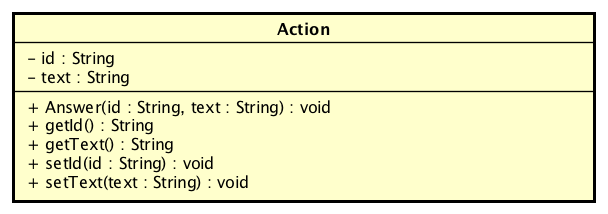
\includegraphics[scale=0.6]{Architettura/Front-End/Models/Action.png}
		\caption{Schema del componente \texttt{Models :: Action}}
	\end{figure}

		\subparagraph{Descrizione}: Rappresenta un'azione predefinita e ne contiene tutte le informazioni necessarie alla presentazione del suo contenuto
		\subparagraph{Utilizzo}: Viene utilizzata per memorizzare i dati di un'azione predefinita
		\subparagraph{Attributi}:
		      \begin{itemize}
		      	\item \texttt{id: string}:
		      	      Attributo che rappresenta l'id di un'azione predefinita.
		      	\item \texttt{text: string}:
		      	      Attributo che rappresenta il testo di un'azione predefinita.
		      \end{itemize}
		\subparagraph{Metodi}:
		      \begin{itemize}
		      	\item \texttt{Action : void}
		      	      \subparagraph{Descrizione}:Costruttore
					\subparagraph{Argomenti}:
						\begin{itemize}
							\item \texttt{id : string}:
								ID dell'Action.
							\item \texttt{text : string}:
								Testo descrittivo dell'Action.
						\end{itemize}

		      	\item \texttt{getId() : string}
		      	      \subparagraph{Descrizione}:Getter dell'ID

		      	\item \texttt{setId() : void}
		      	      \subparagraph{Descrizione}:Setter dell'ID

		      	\item \texttt{setText() : void}
		      	      \subparagraph{Descrizione}:Setter del testo descrittivo

		      	\item \texttt{getText() : string}
		      	      \subparagraph{Descrizione}:Getter del testo descrittivo
		      \end{itemize}



	\newpage
	\subsection{Models :: Admin}
	\begin{figure}[!h]
		\centering
		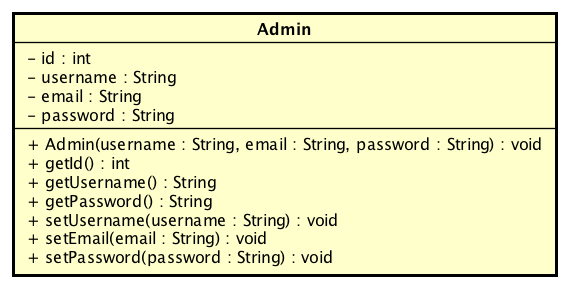
\includegraphics[scale=0.6]{Architettura/Front-End/Models/Admin.png}
		\caption{Schema del componente \texttt{Models :: Admin}}
	\end{figure}

		\subparagraph{Descrizione}: Rappresenta un amministratore e ne contiene tutte le informazioni necessarie alla presentazione del suo contenuto
		\subparagraph{Utilizzo}: Viene utilizzata per memorizzare i dati di un amministratore
		\subparagraph{Attributi}:
		      \begin{itemize}
		      	\item \texttt{email: string}:
		      	      Attributo che rappresenta la email di un amministratore.

		      	\item \texttt{password: string}:
		      	      Attributo che rappresenta la password di un amministratore.

		      	\item \texttt{username: string}:
		      	      Attributo che rappresenta lo username di un amministratore.
		      \end{itemize}
		\subparagraph{Metodi}:
		      \begin{itemize}
		      	\item \texttt{Admin : void}
		      	      \subparagraph{Descrizione}:Costruttore del modello Admin
					\subparagraph{Descrizione}:{Argomenti}:
						\begin{itemize}
							\item \texttt{password : string}:
								Parametro che indica la password dell'amministratore.
							\item \texttt{username : string}:
								Parametro che indica lo username dell'amministratore.
						\end{itemize}

		      	\item \texttt{getEmail : string}:
		      	      \subparagraph{Descrizione}:Funzione che permette di ottenere l'email dell'amministratore

		      	\item \texttt{getPassword : string}:
		      	      \subparagraph{Descrizione}:Funzione che permette di ottenere la password di un amministratore

		      	\item \texttt{getUsername : string}:
		      	      \subparagraph{Descrizione}:Funzione che permette di ottenere lo username di un amministratore

		      	\item \texttt{setEmail}:
		      	     	\subparagraph{Descrizione}: Funzione che permette di modificare la email di un amministratore
					\subparagraph{Argomenti}:
						\begin{itemize}
							\item \texttt{email : string}:
								Parametro che indica la nuova email di un amministratore.
						\end{itemize}

		      	\item \texttt{setPassword}:
		      	     	\subparagraph{Descrizione}: Funzione che permette di modificare la password di un amministratore
					\subparagraph{Argomenti}:
						\begin{itemize}
							\item \texttt{password : string}:
								Parametro che indica la nuova password di un amministratore.
						\end{itemize}

		      	\item \texttt{setUsername(username) : void}:
		      	      \subparagraph{Descrizione}:Funzione che permette di modificare lo username di un amministratore
					\subparagraph{Argomenti}:
						\begin{itemize}
							\item \texttt{username : string}:
								Parametro che indica il nuovo username dell'amministratore.
						\end{itemize}
			\end{itemize}
		      
		\subparagraph{Relazioni con altre classi}:
		      \begin{itemize}
		      	\item \texttt{Front-End :: AdminPage :: AdminComponents :: ManageAdministratorsComponent :: ManageAdministratorsController}: Controller che gestisce la view di ManageAdministrators permettendo ad un SuperAdmin di gestire le informazioni degli altri amministratori;
		      	\item \texttt{Front-End :: AdminPage :: AdminComponents :: ManageProfileComponent :: ManageProfileController}: Controller che gestisce la view di ManageProfileView permettendo ad un amministratore di gestire il proprio profilo nell'area amministrativa.
		      \end{itemize}

	\newpage
	\subsection{Models :: Answer}
	\begin{figure}[!h]
		\centering
		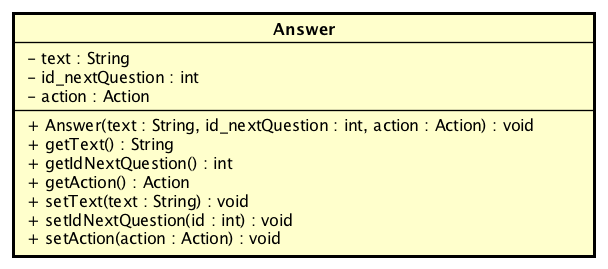
\includegraphics[scale=0.6]{Architettura/Front-End/Models/Answer.png}
		\caption{Schema del componente \texttt{Models :: Answer}}
	\end{figure}

		\subparagraph{Descrizione}: Rappresenta una risposta e ne contiene tutte le informazioni necessarie alla presentazione del suo contenuto
		\subparagraph{Utilizzo}: Viene utilizzata per memorizzare i dati di una risposta
		\subparagraph{Attributi}:
		      \begin{itemize}
		      	\item \texttt{action: Action}:
		      	      Attributo che rappresenta l'azione predefinita da eseguire legata ad una risposta.

		      	\item \texttt{id\_nextQuestion: int}:
		      	      Attributo che rappresenta l'id della prossima domanda legata ad una risposta.

		      	\item \texttt{text: string}:
		      	      Attributo che rappresenta il testo di una risposta.
		      \end{itemize}
		\subparagraph{Metodi}:
		      \begin{itemize}
		      	\item \texttt{Answer}:
		      	      \subparagraph{Descrizione}:Costruttore
					\subparagraph{Descrizione}{Argomenti}:
						\begin{itemize}
							\item \texttt{action : Action}:
								Azione da eseguire.
							\item \texttt{text : string}:
								Testo della risposta.
						\end{itemize}
		     
		      	\item \texttt{getAction : Action}:
		      	      \subparagraph{Descrizione}:Getter dell'azione da eseguire

		      	\item \texttt{getIdNextQuestion : int}:
		      	      \subparagraph{Descrizione}:Getter dell'ID della prossima domanda da porre
		      
		      	\item \texttt{getText : string}:
		      	      \subparagraph{Descrizione}:Getter del testo
		      
		      	\item \texttt{setAction : void}:
		      	      \subparagraph{Descrizione}:Setter dell'Action

		      	\item \texttt{setIdNextQuestion : void}:
		      	      \subparagraph{Descrizione}: Setter dell'ID della prossima domanda da porre
					\subparagraph{Argomenti}:
						\begin{itemize}
							\item \texttt{id : int}:
								ID della prossima domanda.
						\end{itemize}

		      	\item \texttt{setText() : void}:
		      	      \subparagraph{Descrizione}: Setter del testo della risposta
		      \end{itemize}\vspace{0.5em}
		\subparagraph{Relazioni con altre classi}:
		      \begin{itemize}
		      	\item \texttt{Front-End :: AdminPage :: AdminComponents :: ManageQuestionsComponent :: ManageQuestionsController}: Componente per le domande e interazioni.
		      \end{itemize}


\newpage
	\subsection{Models :: Conversation}
	\begin{figure}[!h]
		\centering
		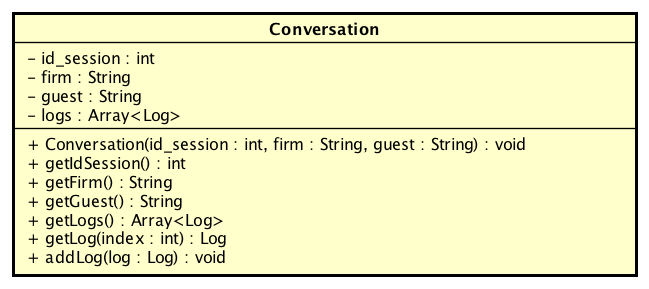
\includegraphics[scale=0.6]{Architettura/Front-End/Models/Conversation.png}
		\caption{Schema del componente \texttt{Models :: Conversation}}
	\end{figure}
		\subparagraph{Descrizione}: Rappresenta una conversazione e ne contiene tutte le informazioni necessarie alla presentazione del suo contenuto
		\subparagraph{Utilizzo}: Viene utilizzata per memorizzare i dati di una conversazione
		\subparagraph{Attributi}:
				\begin{itemize}
					\item \texttt{id\_session: int}: Attributo che rappresenta la session\_id di un conversazione.

					\item \texttt{firm: string}: Attributo che rappresenta il nome dell'azienda

					\item \texttt{guest : string}: Attributo che rappresenta il nominativo di un ospite

					\item \texttt{logs: Array<Log>}: Attributo che rappresenta l'insieme dei log di una conversazione
				\end{itemize}
			\subparagraph{Metodi}:
				\begin{itemize}
					\item \texttt{addLog : void}:
					      \subparagraph{Descrizione}:Funzione che permette di aggiungere un log alla conversazione
						\subparagraph{Argomenti}:
							\begin{itemize}
								\item \texttt{log : Log}:
									Parametro che indica il nuovo log da aggiungere alla conversazione.
							\end{itemize}

					\item \texttt{Conversation : void}:
					      \subparagraph{Descrizione}: Costruttore del model Conversation
						\subparagraph{Argomenti}:
							\begin{itemize}
								\item \texttt{id\_session : int}:
									Parametro che indica l'id\_session della sessione di Alexa.
							\end{itemize}

					\item \texttt{getIdSession : int}:
					      \subparagraph{Descrizione}:Funzione che permette di ottenere l'id\_session di una conversazione

					\item \texttt{getLog : Log}:
					     \subparagraph{Descrizione}: Funzione che permette di ottenere uno specifico log di una conversazione
	
					\item \texttt{getLogs : Array<Log>}: 
						\subparagraph{Descrizione}:Funzione che permette di ottenere l'insieme dei log di una conversazione

					\item \texttt{getFirm : string}: 
						\subparagraph{Descrizione}:Funzione che permette di ottenere il nome dell'azienda

					\item \texttt{getGuest : string}: 
						\subparagraph{Descrizione}:Funzione che permette di ottenere il nome di un ospite
				\end{itemize}

		\subparagraph{Relazioni con altre classi}:
		      \begin{itemize}
		      	\item \texttt{Front-End :: AdminPage :: AdminComponents :: ManageFirmsComponent :: ManageFirmsController}: Componente per la scelta degli oggetti di tipo Firm.
		      \end{itemize}

\newpage
	\subsection{Models :: Firm}
	\begin{figure}[!h]
		\centering
		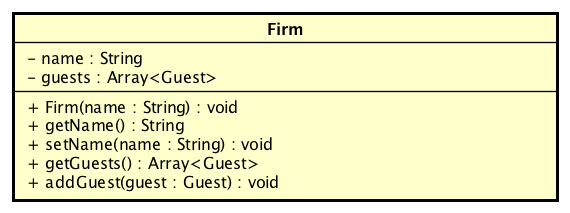
\includegraphics[scale=0.6]{Architettura/Front-End/Models/Firm.png}
		\caption{Schema del componente \texttt{Models :: Firm}}
	\end{figure}

		
		\subparagraph{Descrizione}: Rappresenta un'azienda e ne contiene tutte le informazioni necessarie alla presentazione del suo contenuto
		
		\subparagraph{Utilizzo}: Viene utilizzata per memorizzare i dati di un'azienda
		
		\subparagraph{Attributi}:
		      \begin{itemize}
		      	\item \texttt{guests: Array<Guest>}:
		      	      Attributo che rappresenta gli ospiti registrati di un'azienda.
		      	\item \texttt{id: int}:
		      	      Attributo che rappresenta l'id di un'azienda.
		      	\item \texttt{name: string}:
		      	      Attributo che rappresenta il nome di un'azienda.
		      \end{itemize}
		
		\subparagraph{Metodi}:
		      \begin{itemize}
		      	\item \texttt{addGuest}:
		      	      \subparagraph{Descrizione}:Funzione che permette di aggiungere un nuovo ospiti ad un'azienda
		      	\subparagraph{Argomenti}:
		      	      \begin{itemize}
		      	      	\item \texttt{guest : Guest}:
		      	      	      Parametro che indica l'ospite da aggiungere all'azienda.
		      	      \end{itemize}

		      	\item \texttt{Firm}:
		      	      \subparagraph{Descrizione}:Costruttore del model azienda
		      	\subparagraph{Argomenti}:
		      	      \begin{itemize}
		      	      	\item \texttt{name : string}:
		      	      	      Parametro che indica il nome di un'azienda.
		      	      \end{itemize}

		      	\item \texttt{getId : int}:
		      	      \subparagraph{Descrizione}Funzione che permette di ottenere l'id di un'azienda

		      	\item \texttt{getName : string}:
		      	      \subparagraph{Descrizione}Funzione che permette di ottenere il nome di un'azienda

		      	\item \texttt{setName}:
		      	      \subparagraph{Descrizione}Funzione che permette di modificare il nome di un'azienda
		      		\subparagraph{Argomenti}:
		      	      \begin{itemize}
		      	      	\item \texttt{name : string}:
		      	      	      Parametro che indica il nuovo nome dell'azienda.
		      	      \end{itemize}
		      \end{itemize}
		\subparagraph{Relazioni con altre classi}:
		      \begin{itemize}
		      	\item \texttt{Front-End :: AdminPage :: AdminComponents :: ManageFirmsComponent :: ManageFirmsController}: Componente per la scelta degli oggetti di tipo Firm.
		      \end{itemize}


	\newpage
	\subsection{Models :: Guest}
	\begin{figure}[!h]
		\centering
		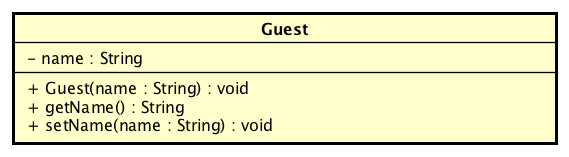
\includegraphics[scale=0.6]{Architettura/Front-End/Models/Guest.png}
		\caption{Schema del componente \texttt{Models :: Guest}}
	\end{figure}

		\subparagraph{Descrizione}: Rappresenta un ospite e ne contiene tutte le informazioni necessarie alla presentazione del suo contenuto
		\subparagraph{Utilizzo}: Viene utilizzata per memorizzare i dati di un ospite
		\subparagraph{Attributi}:
		      \begin{itemize}
		      	\item \texttt{name: string}:
		      	      Attributo che rappresenta il nome di un ospite
		      	      .
		      \end{itemize}
		\subparagraph{Metodi}:
		      \begin{itemize}
		      	\item \texttt{getName : string}:
		      	      \subparagraph{Descrizione}:Funzione che permette di ottenere il nome di un guest

		      	\item \texttt{Gues : void}:
		      	     \subparagraph{Descrizione}: Costruttore del modello Guest

		      	\item \texttt{setName : void}:
		      	      \subparagraph{Descrizione}:Funzione che permette di modificare il nome di un ospite
		      \end{itemize}

		\subparagraph{Relazioni con altre classi}:
		      \begin{itemize}
		      	\item \texttt{Front-End :: AdminPage :: AdminComponents :: ManageFirmsComponent :: ManageFirmsController}: Componente per la scelta degli oggetti di tipo Firm.
		      \end{itemize}

	\newpage
	\subsection{Models :: Interlocutor}
	\begin{figure}[!h]
		\centering
		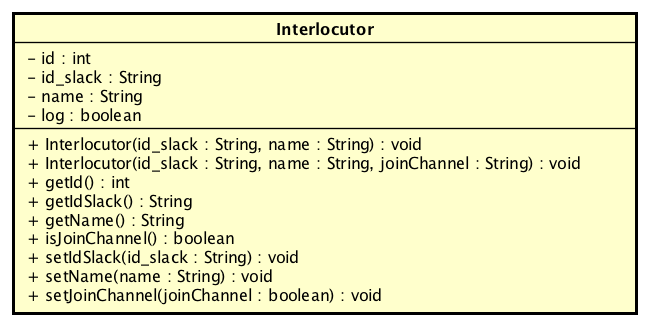
\includegraphics[scale=0.6]{Architettura/Front-End/Models/Interlocutor.png}
		\caption{Schema del componente \texttt{Models :: Interlocutor}}
	\end{figure}

		\subparagraph{Descrizione}: Rappresenta un interlocutore e ne contiene tutte le informazioni necessarie alla presentazione del suo contenuto
		\subparagraph{Utilizzo}: Viene utilizzata per memorizzare i dati di un interlocutore
		\subparagraph{Attributi}:
			\begin{itemize}
				\item \texttt{id\_slack: string}: Attributo che rappresenta l'id di Slack di un interlocutore

				\item \texttt{default: boolean}: Attributo che indica se un interlocutore è associato o meno alla lista di default \#azienda.

				\item \texttt{name: string}: Attributo che rappresenta il nome di un interlocutore
			\end{itemize}
			\subparagraph{Metodi}:
			\begin{itemize}
				\item \texttt{getSlackId : string}
				      \subparagraph{Descrizione}: Funzione che permette di ottenere l'id\_slack di un interlocutore

				\item \texttt{getName : string}
				      \subparagraph{Descrizione}:Funzione che permette di ottenere il nome di un interlocutore

				\item \texttt{Interlocutor}
				      \subparagraph{Descrizione}:Costruttore del modello Interlocutor
					\subparagraph{Argomenti}:
						\begin{itemize}
							\item \texttt{id\_slack : string}:
								Parametro che indica l'id Slack dell'interlocutore.
						\end{itemize}

				\item \texttt{Interlocutor}
				      \subparagraph{Descrizione}: Costruttore del modello Interlocutor
					\subparagraph{Argomenti}:
						\begin{itemize}
							\item \texttt{id\_slack : string}:
								Parametro che indica l'id Slack dell'interlocutore.
						\end{itemize}

				\item \texttt{setIdSlack}
				      \subparagraph{Descrizione}:Funzione che permette di modificare l'id\_slack di un interlocutore
					\subparagraph{Argomenti}:
				      \begin{itemize}
				      	\item \texttt{id\_slack : string}:
				      	      Parametro che indica il nuovo id\_slack di un interlocutore.
				      \end{itemize}

				\item \texttt{setDefault}
				      \subparagraph{Descrizione}Funzione che permette di modificare l'associazione di un interlocutore alla lista di default \#azienda
					\subparagraph{Argomenti}:
						\begin{itemize}
							\item \texttt{joinChannel : boolean}:
								Parametro che indica l'associazione o meno di un interlocutore alla lista di default \#azienda.
						\end{itemize}

				\item \texttt{setName}:
				      \subparagraph{Descrizione}:Funzione che permette di modificare il nome di un interlocutore

				\item \texttt{isDefault}:
				      \subparagraph{Descrizione}:Funzione che permette di sapere se un interlocutore è associato alla lista di default \#azienda
			\end{itemize}\vspace{0.5em}

			\subparagraph{Relazioni con altre classi}:
			\begin{itemize}
				\item \texttt{Front-End :: AdminPage :: AdminComponents :: ManageSlackComponent :: ManageSlackController}: Componente per la gestione dei canali Slack.
			\end{itemize}


	\newpage
	\subsection{Models :: Log}
	\begin{figure}[!h]
		\centering
		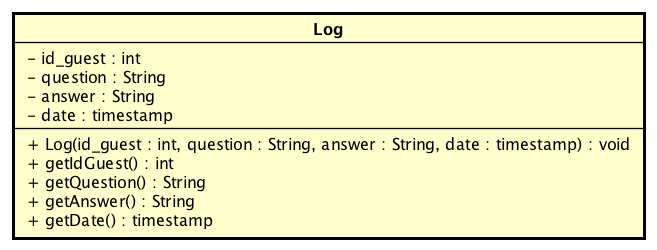
\includegraphics[scale=0.6]{Architettura/Front-End/Models/Log.png}
		\caption{Schema del componente \texttt{Models :: Log}}
	\end{figure}

		\subparagraph{Descrizione}: Rappresenta un log e ne contiene tutte le informazioni necessarie alla presentazione del suo contenuto
		\subparagraph{Utilizzo}: Viene utilizzata per memorizzare i dati di un log
		\subparagraph{Attributi}:
		      \begin{itemize}
		      	\item \texttt{answer: string}:
		      	      Attributo che rappresenta la risposta legata ad un log.
		     
		      	\item \texttt{date: string}:
		      	      Attributo che rappresenta la data legata ad un log.

		      	\item \texttt{id\_guest: int}:
		      	      Attributo che rappresenta l'id dell'ospite in un log.

		      	\item \texttt{question: string}:
		      	      Attributo che rappresenta la domanda legata ad un log.
		      \end{itemize}
		\subparagraph{Metodi}:
		      \begin{itemize}
		      	\item \texttt{getAnswer : string}
		      	      \subparagraph{Descrizione}:Funzione che permette di ottenere il testo della risposta legato ad un log

		      	\item \texttt{getDate : string}
		      	      \subparagraph{Descrizione}:Funzione che permette di ottenere la data legata ad un log

		      	\item \texttt{getDate : string}:
		      	      Getter del timestamp del log

		      	\item \texttt{getIdGuest : int}
		      	      \subparagraph{Descrizione}: Funzione che permette di ottenere l'id\_guest legato ad un log

		      	\item \texttt{getQuestion : string}
		      	      \subparagraph{Descrizione}: Funzione che permette di ottenere il testo della domanda legato ad un log

		      	\item \texttt{Log}:
		      	      \subparagraph{Descrizione}:Costruttore del modello Log
					\subparagraph{Argomenti}:
						\begin{itemize}
							\item \texttt{date : string}:
								Parametro che indica la data legata al log.
							\item \texttt{id\_guest : int}:
								Parametro che indica l'id\_guest legato al Log.
							\item \texttt{question : string}:
								Parametro che indica il testo della domanda legata al log.
						\end{itemize}
		      \end{itemize}

		\subparagraph{Relazioni con altre classi}:
		      \begin{itemize}
		      	\item \texttt{Front-End :: AdminPage :: AdminComponents :: ManageFirmsComponent :: ManageFirmsController}: Componente per la scelta degli oggetti di tipo Firm.
		      \end{itemize}

	\newpage
	\subsection{Models :: Question}
	\begin{figure}[!h]
		\centering
		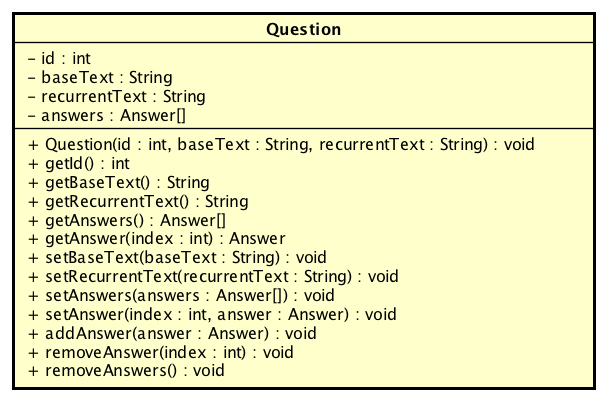
\includegraphics[scale=0.6]{Architettura/Front-End/Models/Question.png}
		\caption{Schema del componente \texttt{Models :: Question}}
	\end{figure}

		\subparagraph{Descrizione}: Rappresenta una domanda e ne contiene tutte le informazioni necessarie alla presentazione del suo contenuto
		\subparagraph{Utilizzo}: Viene utilizzata per memorizzare i dati di una domanda
		\subparagraph{Attributi}:
		      \begin{itemize}
		      	\item \texttt{answers: Answer[]}:
		      	      Attributo che rappresenta l'insieme delle risposte allegate ad una domanda.

		      	\item \texttt{baseText: string}:
		      	      Attributo che rappresenta il testo base di una domanda.

		      	\item \texttt{id: int}:
		      	      Attributo che rappresenta l'id di una domanda.

		      	\item \texttt{recurrentText: string}:
		      	      Attributo che rappresenta il testo ricorrente di una domanda.
		      \end{itemize}
		\subparagraph{Metodi}:
		      \begin{itemize}
		      	\item \texttt{addAnswer}
		      	      \subparagraph{Descrizione}:Aggiunge una risposta
		      	\subparagraph{Argomenti}:
		      	      \begin{itemize}
		      	      	\item \texttt{answer : Answer}:
		      	      	      Risposta.
		      	      \end{itemize}

		      	\item \texttt{getAnswer : Action}
		      	      \subparagraph{Descrizione}Ricerca di una riposta tramite indice
		      	\subparagraph{Argomenti}:
		      	      \begin{itemize}
		      	      	\item \texttt{index : int}:
		      	      	      Indice della risposta.
		      	      \end{itemize}

		      	\item \texttt{getAnswers : Answer[]}
		      	      \subparagraph{Descrizione}:Getter delle risposte

		      	\item \texttt{getBaseText : string}
		      	      \subparagraph{Descrizione}:Getter del testo base

		      	\item \texttt{getId : int}
		      	      \subparagraph{Descrizione}:Getter dell'ID della domanda

		      	\item \texttt{getRecurrentText : string}
		      	      \subparagraph{Descrizione}:Getter del testo ricorrente

		      	\item \texttt{Question}
		      	      \subparagraph{Descrizione}:Costruttore
					\subparagraph{Argomenti}:
						\begin{itemize}
							\item \texttt{id : int}:
								Id della domanda.
						\end{itemize}

		      	\item \texttt{removeAnswer}
		      	      \subparagraph{Descrizione}:Rimuove una domanda
					\subparagraph{Argomenti}:
						\begin{itemize}
							\item \texttt{index : int}:
								indice della domanda da rimuovere.
						\end{itemize}

		      	\item \texttt{removeAnswers}
		      	      \subparagraph{Descrizione}:Rimuove tutte le risposte

		      	\item \texttt{setAnswer}
		      	      \subparagraph{Descrizione}:Setter di una risposta

		      	\item \texttt{setAnswers}
		      	      \subparagraph{Descrizione}:Setter delle risposte

		      	\item \texttt{setBaseText}
		      	      \subparagraph{Descrizione}:Setter del testo base

		      	\item \texttt{setRecurrentText(recurrentText)}
		      	      \subparagraph{Descrizione}:Setter del testo ricorrente
					\subparagraph{Argomenti}:
						\begin{itemize}
							\item \texttt{recurrentText : string}:
								Testo ricorrente.
						\end{itemize}
		      \end{itemize}\vspace{0.5em}
		\subparagraph{Relazioni con altre classi}:
		      \begin{itemize}
		      	\item \texttt{Front-End :: AdminPage :: AdminComponents :: ManageQuestionsComponent :: ManageQuestionsController}: Componente per le domande e interazioni.
		      \end{itemize}

\end{document}